\chapter[Resultados]{Resultados}

	Para cada \textit{shader} foram plotados os gráficos para a métrica de vértice e para a de fragmento. Após as plotagens, percebeu-se que todos os gráficos de todos os \textit{shaders} relacionados ao vértice deram uma função linear (diferindo na inclinação), e os relacionados ao fragmento deram uma curva de formato semelhante. A Figura \ref{plotred}, Figura \ref{plottoon}, Figura \ref{plotphong}, Figura \ref{plotgou}, Figura \ref{plotrefl}, Figura \ref{plotcube}, Figura \ref{plotflat}, Figura \ref{plottex} e Figura \ref{plotcolor}  mostram os gráficos plotados, com relação ao \textit{vertex} e \textit{fragment shaders} de cada \textit{shader} implementado, que demonstram a semelhança das curvas

	\begin{figure}[h]
	\centering
		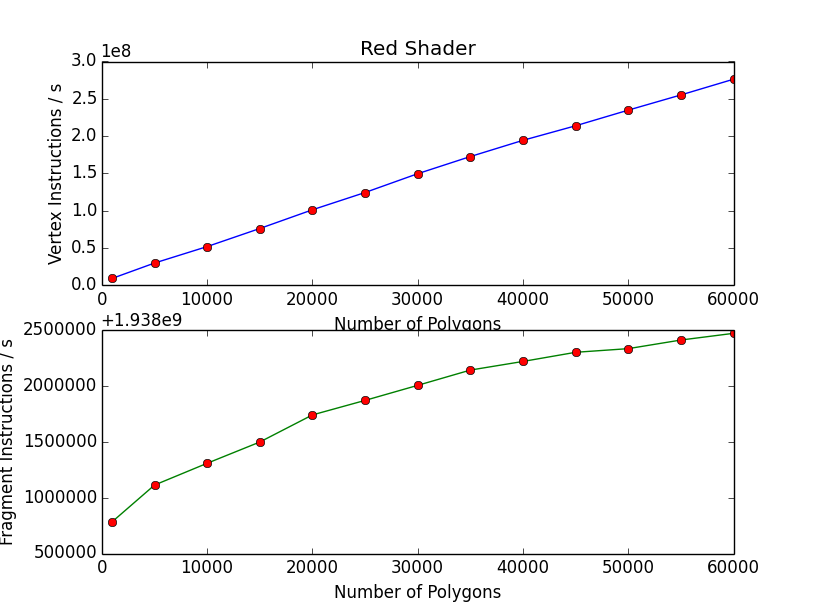
\includegraphics[keepaspectratio=true,scale=0.6]{figuras/red.png}
	\caption{Gráficos: \textit{red shader}}
	\label{plotred}
	\end{figure}
 
	\begin{figure}[h]
	\centering
		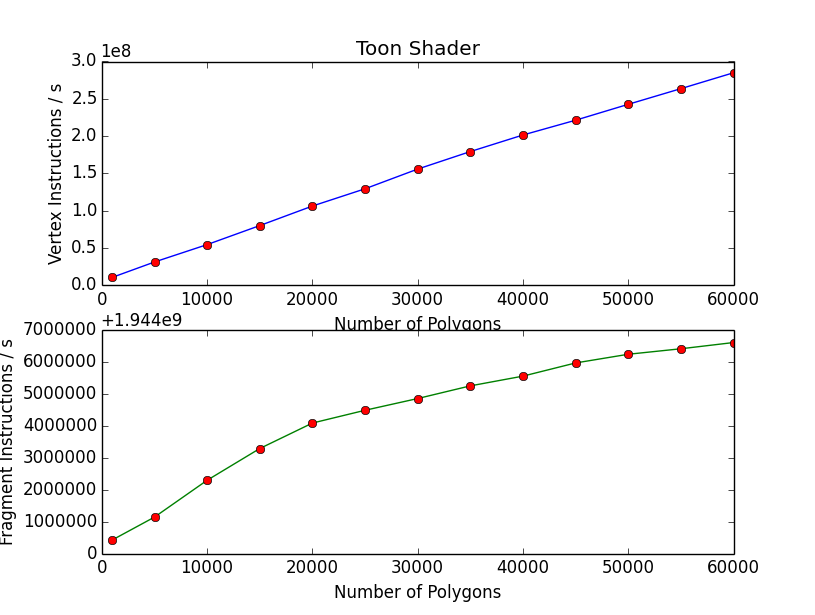
\includegraphics[keepaspectratio=true,scale=0.6]{figuras/toonplot.png}
	\caption{Gráficos: \textit{toon shader}}
	\label{plottoon}
	\end{figure}	

	\begin{figure}[h]
	\centering
		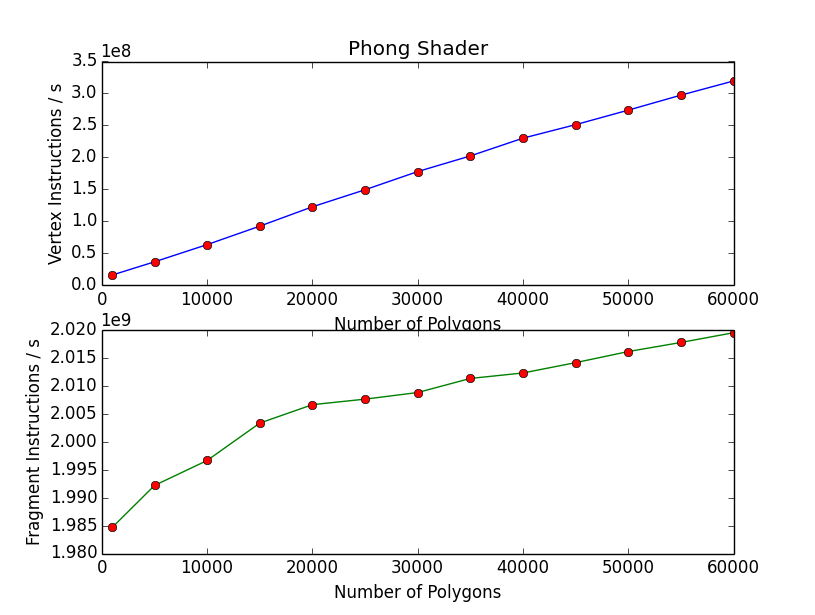
\includegraphics[keepaspectratio=true,scale=0.6]{figuras/phongplot.png}
	\caption{Gráficos: \textit{phong shader}}
	\label{plotphong}
	\end{figure}

	\begin{figure}[h]
	\centering
		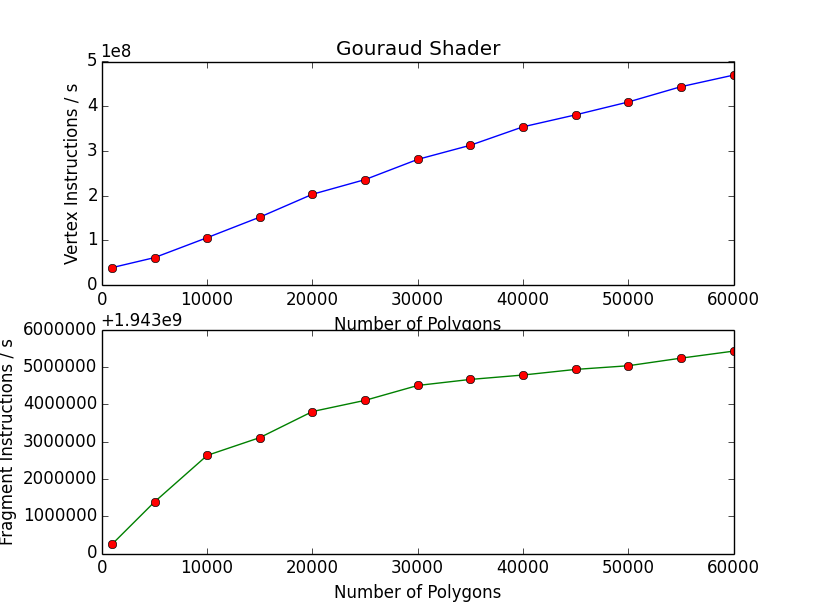
\includegraphics[keepaspectratio=true,scale=0.6]{figuras/gouplot.png}
	\caption{Gráficos: \textit{gouraud shader}}
	\label{plotgou}
	\end{figure}
 
	\begin{figure}[h]
	\centering
		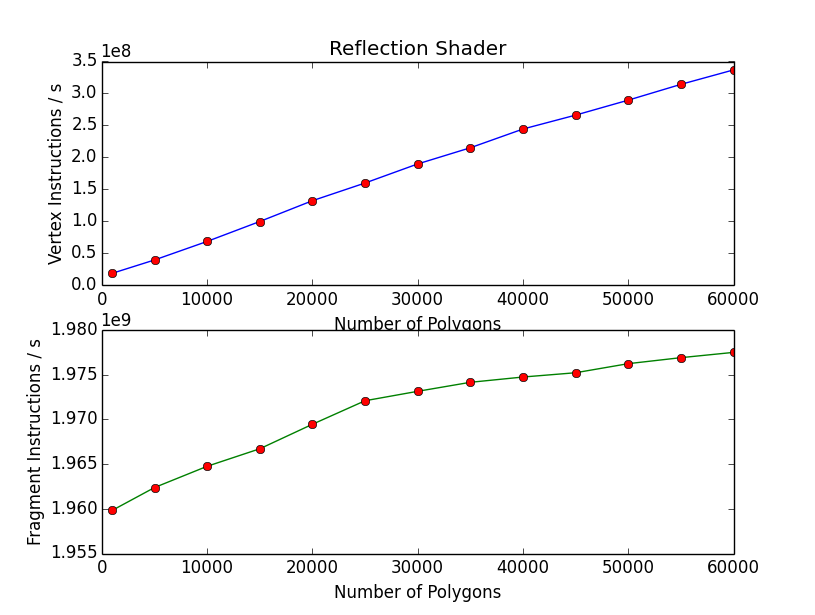
\includegraphics[keepaspectratio=true,scale=0.6]{figuras/reflectionplot.png}
	\caption{Gráficos: \textit{reflection shader}}
	\label{plotrefl}
	\end{figure}

	\begin{figure}[h]
	\centering
		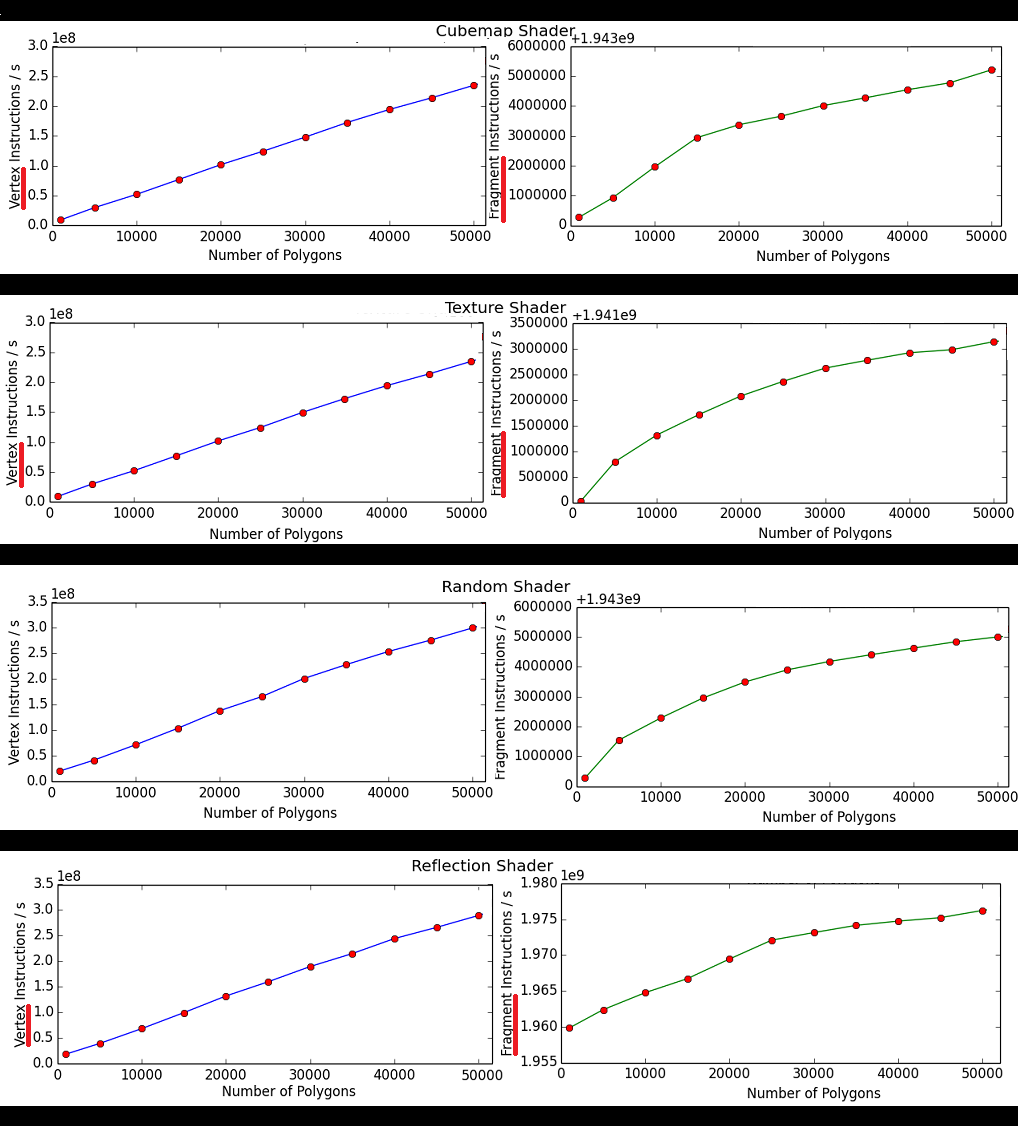
\includegraphics[keepaspectratio=true,scale=0.6]{figuras/cubeplot.png}
	\caption{Gráficos: \textit{cube map shader}}
	\label{plotcube}
	\end{figure}

	\begin{figure}[h]
	\centering
		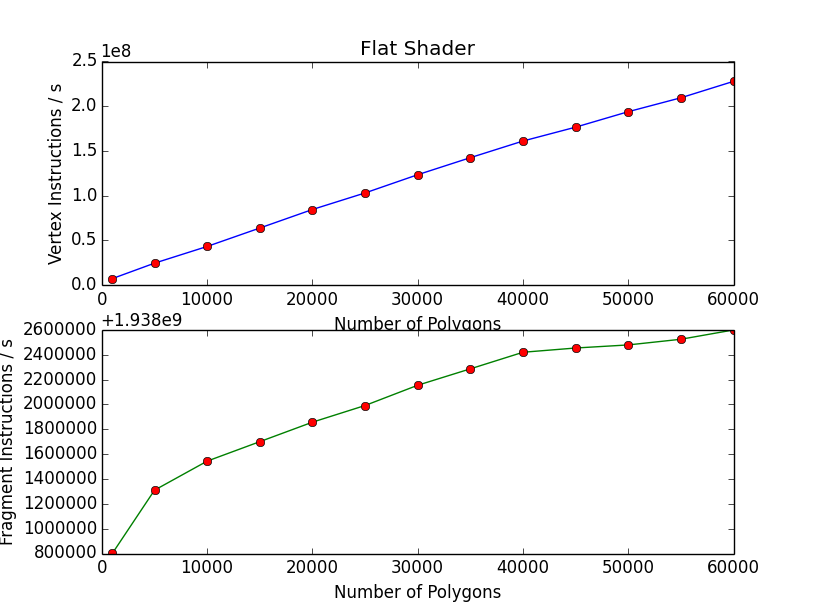
\includegraphics[keepaspectratio=true,scale=0.6]{figuras/flatplot.png}
	\caption{Gráficos: \textit{flat shader}}
	\label{plotflat}
	\end{figure}

	\begin{figure}[h]
	\centering
		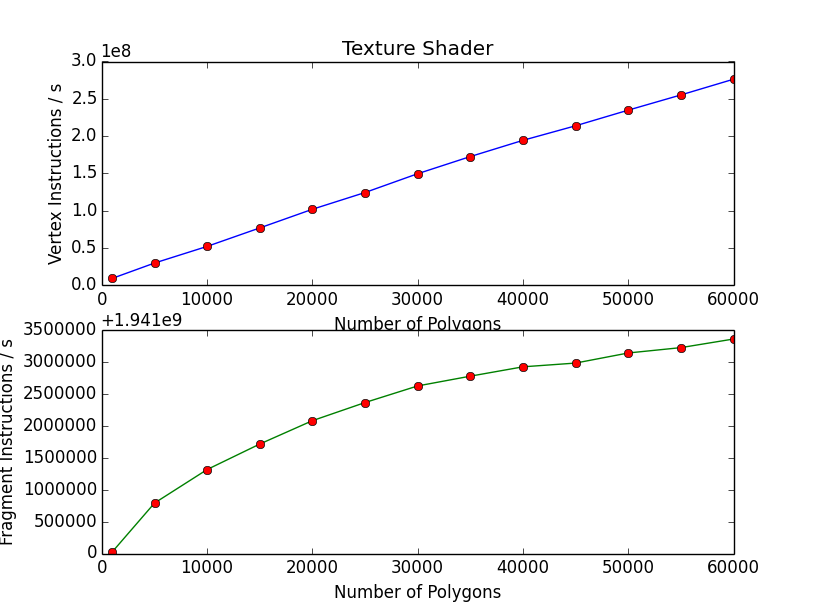
\includegraphics[keepaspectratio=true,scale=0.6]{figuras/texplot.png}
	\caption{Gráficos: \textit{simple texture shader}}
	\label{plottex}
	\end{figure}

	\begin{figure}[h]
	\centering
		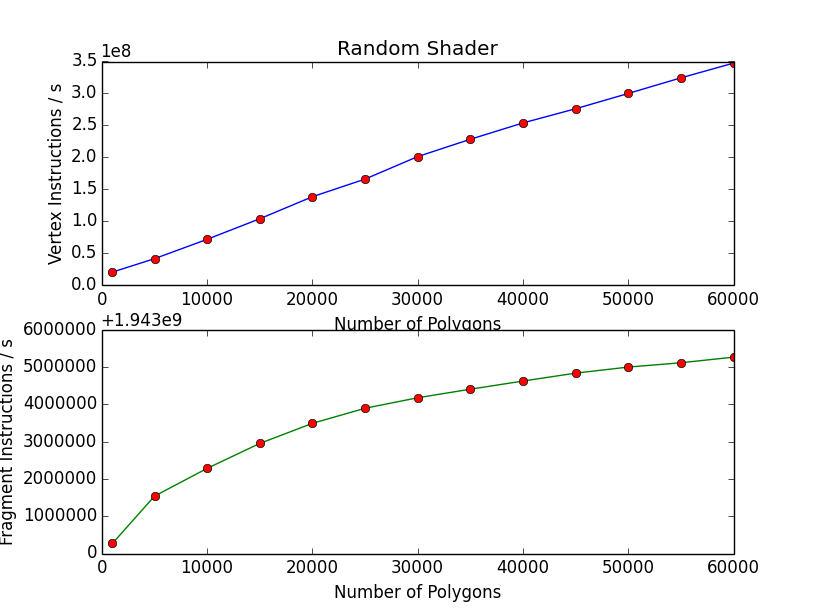
\includegraphics[keepaspectratio=true,scale=0.6]{figuras/randomplot.png}
	\caption{Gráficos: \textit{random shader}}
	\label{plotcolor}
	\end{figure}

	 Os ajustes de cada curva (linear, exponencial, segundo e terceiro graus) também foram plotados (Figura \ref{linear}, Figura \ref{exp}, Figura \ref{sec} e Figura \ref{third} referentes ao \textit{reflection shader}), em que avisa-se qual foi o menor erro associado. Pela a análise do menor erro, calculado de acordo com a Seção \ref{metminqua}, todos os \textit{shaders} indicaram uma curva de segundo grau.

	\begin{figure}[h]
	\centering
		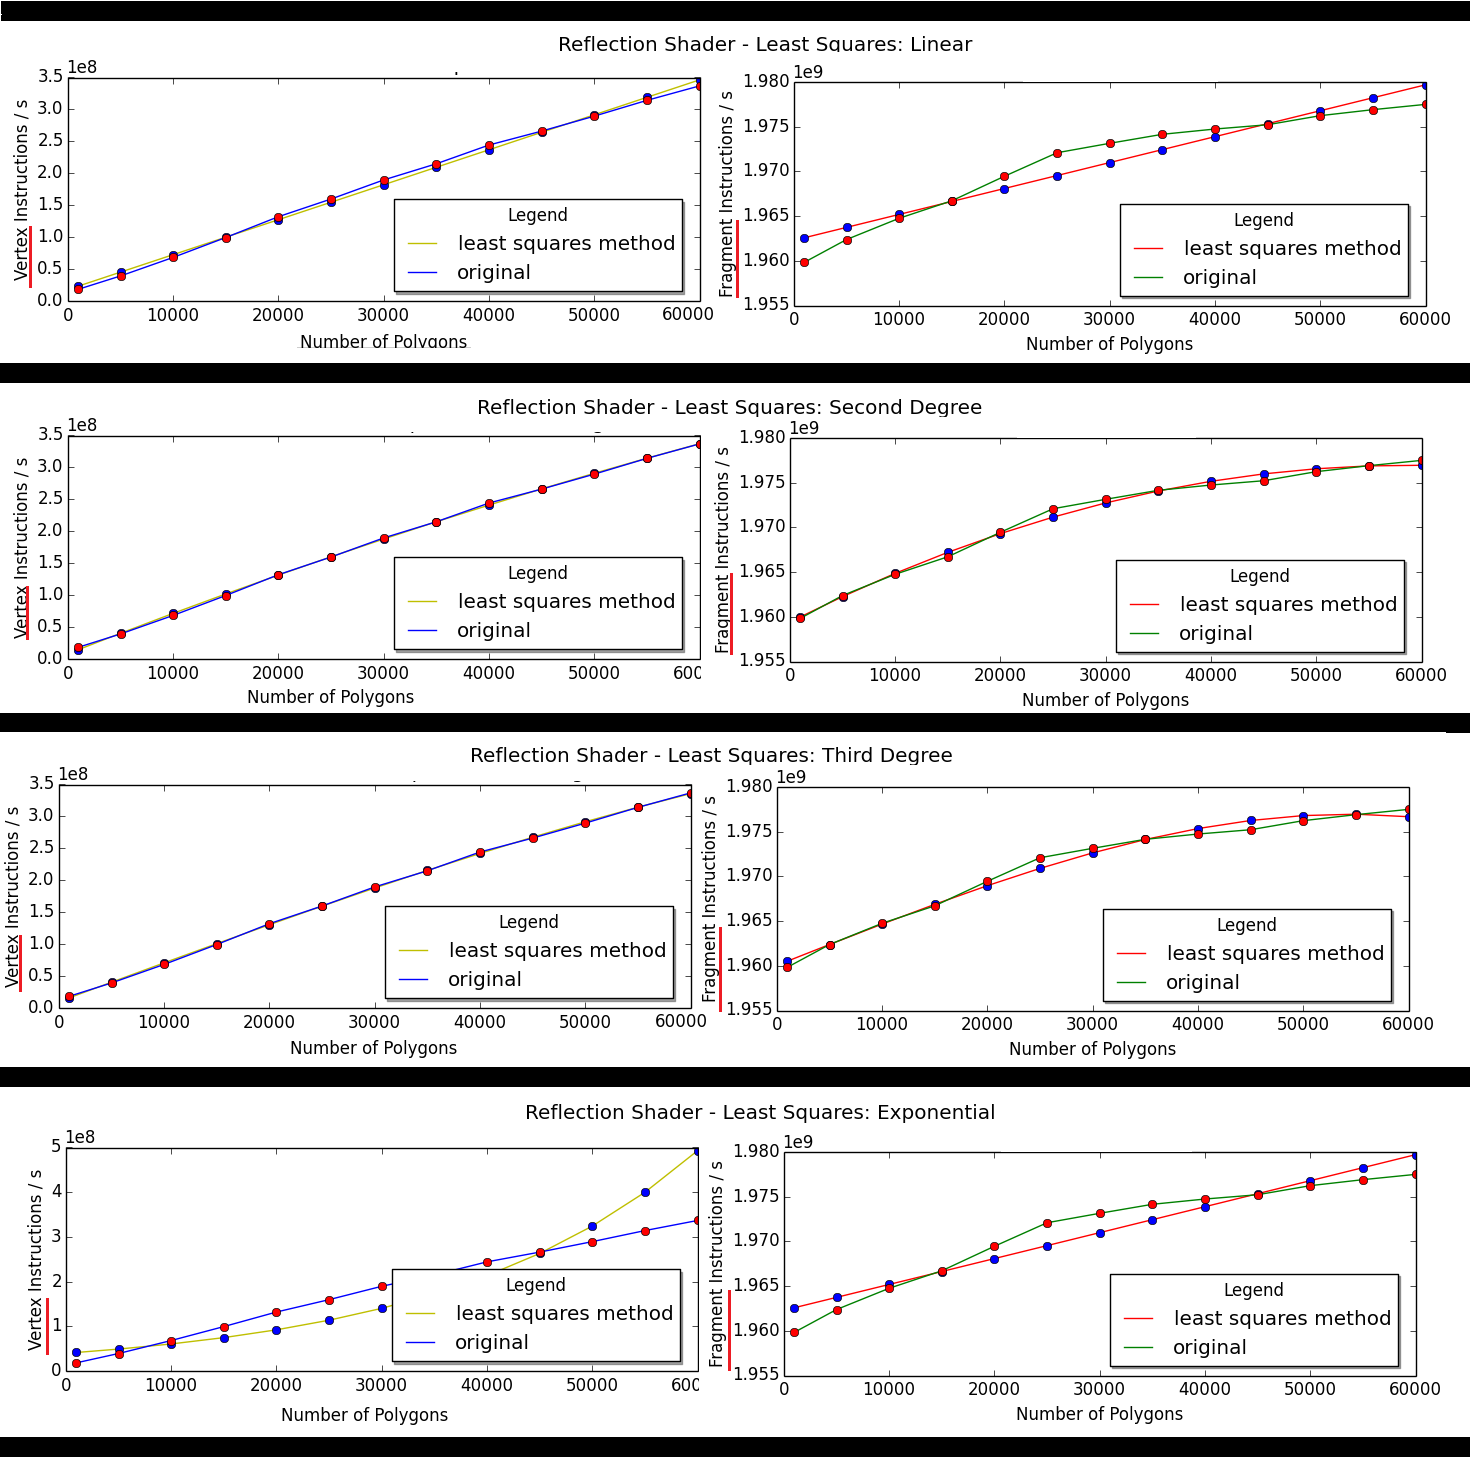
\includegraphics[keepaspectratio=true,scale=0.4]{figuras/reflectionlinear.png}
	\caption{Ajuste linear}
	\label{linear}
	\end{figure}	

	\begin{figure}[h]
	\centering
		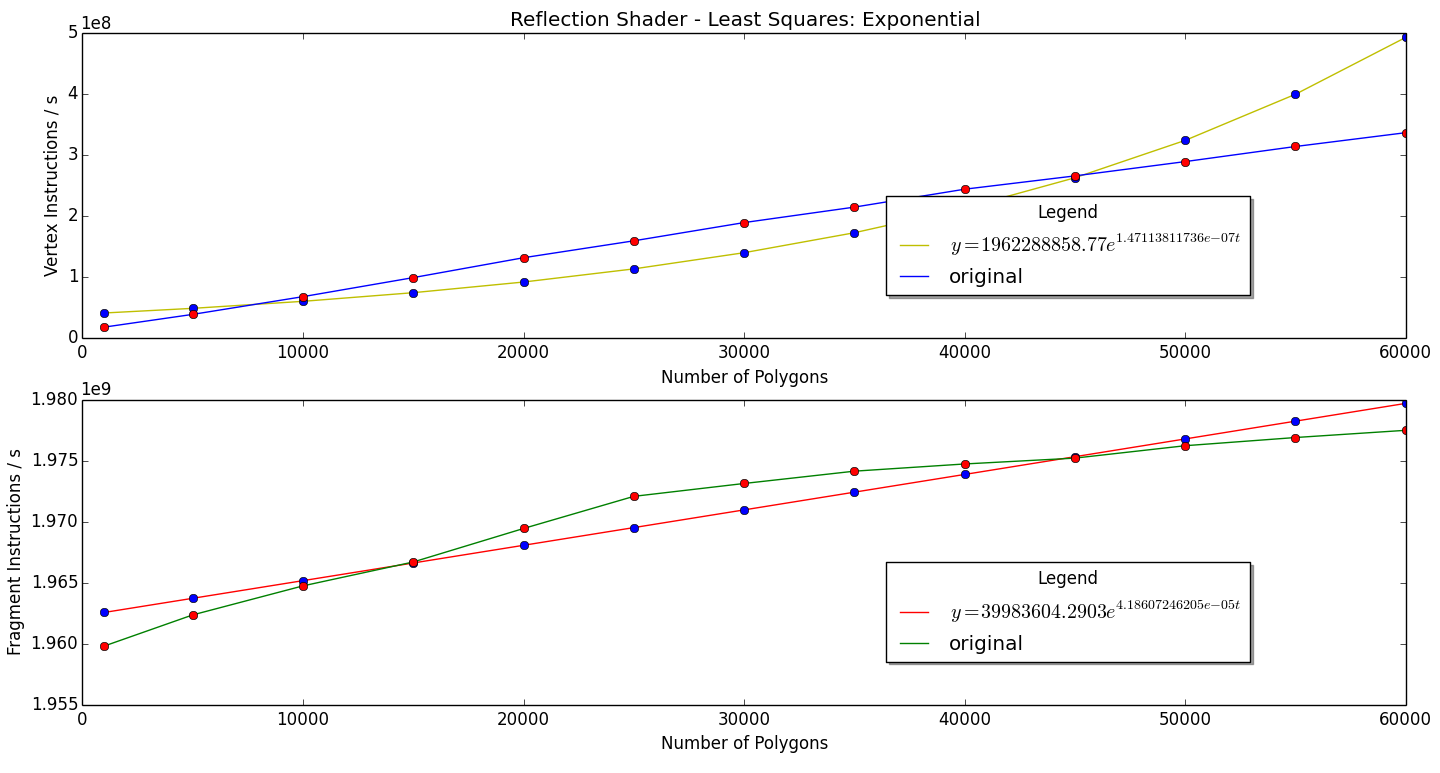
\includegraphics[keepaspectratio=true,scale=0.4]{figuras/reflectionexponential.png}
	\caption{Ajuste exponencial}
	\label{exp}
	\end{figure}	

	\begin{figure}[h]
	\centering
		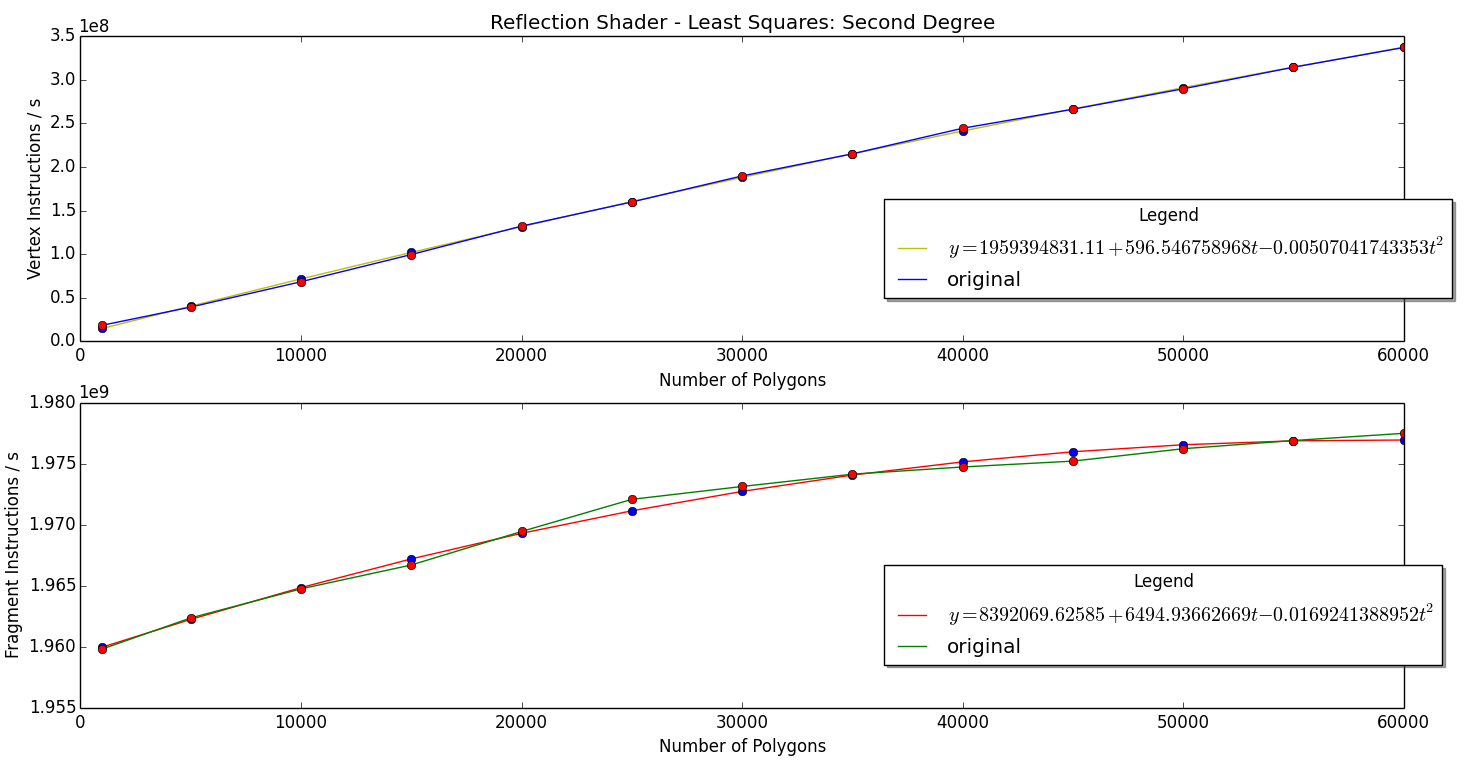
\includegraphics[keepaspectratio=true,scale=0.4]{figuras/reflectionsec.png}
	\caption{Ajuste função de segundo grau}
	\label{sec}
	\end{figure}	

	\begin{figure}[h]
	\centering
		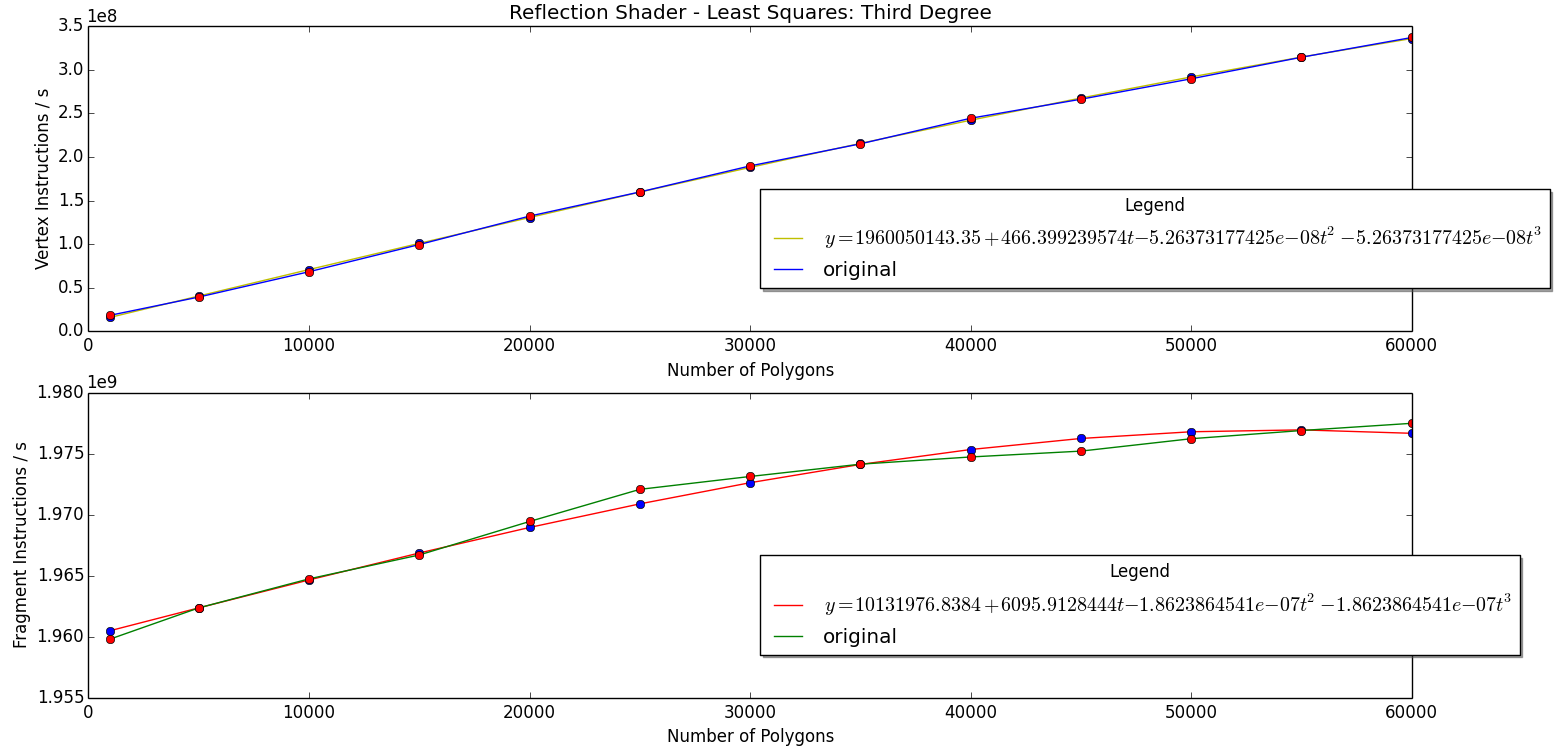
\includegraphics[keepaspectratio=true,scale=0.4]{figuras/reflectionthird.png}
	\caption{Ajuste função de terceiro grau}
	\label{third}
	\end{figure}	

	As equações calculadas para cada \textit{shader} (relacionadas ao vértice e fragmento) são mostradas na Tabela \ref{equacoes}.

	\begin{table}[h]
	\centering	
	\begin{tabularx}{0.9\textwidth}{cXX}
		\toprule
		\textbf{Nome} & \textbf{\textit{Equação Vertex Shader}} & \textbf{\textit{Equação Fragment Shader}}  \\
		\midrule
		\textit{Gouraud} & $y = 19.92 x 10^8 + 509.43t$ & $y = 67.99 x 10 ^5 + 6076.30t - 0.014t^2$ \\
		\textit{Phong} &  $y = 19.45 x 10^8 + 74.85t$ & $y = 20.20 x 10^6 + 9605.32t - 0.035t^2$\\
		\textit{Red} & $y = 19.39 x 10^8 + 26.84t$ & $y = 29.95 x 10 ^5 + 5130.50t - 0.0097t^2$ \\
		\textit{Toon} & $y = 19.45 x 10^8 + 100.35t$ & $y = 38.25 x 10 ^5 + 5347.86t - 0.011t^2$ \\
		\textit{Flat} & $y = 19.39 x 10^8 + 26.77t$ & $y = 25.02 x 10 ^5 + 4285.80t - 0.0091t^2$ \\
		\textit{Random Color} & $y = 19.45 x 10^8 + 74.04t$ & $y = 84.32 x 10 ^5 + 6930.50t - 0.021t^2$ \\
		\textit{Simple Texture} & $y = 19.42 x 10^8 + 49.97t$ & $y = 31.76 x 10 ^5 + 5137.26t - 0.0099t^2$ \\
		\textit{CubeMap} & $y = 19.44 x 10^8 + 83.38t$ & $y = 33.14 x 10 ^5 + 5109.61t - 0.0094t^2$ \\
		\textit{Reflection} & $y = 19.62 x 10^8 + 289.76t$ & $y = 83.92 x 10 ^5 + 6494.94t - 0.017t^2$ \\
	
		\bottomrule
	\end{tabularx}
	\caption{Equações relacionadas ao \textit{vertex shader} e \textit{fragment shader}}
	\label{equacoes}
	\end{table}
